\documentclass{beamer}

\usetheme{Warsaw} 
\usecolortheme{default}

\usepackage[utf8]{inputenc}
\usepackage{graphicx}
\usepackage{amsmath}

\logo{
\includegraphics[width=1.2cm]{unisi-logo}}

\title{Seminar Presentation}
\subtitle{University Course}
\author{Presenter's Name}
\institute{University of Siena}
\date{\today}

\begin{document}
	\begin{frame}
		\titlepage
	\end{frame}
	
	\begin{frame}{Seminar Outline}
		\begin{itemize}
			\item Introduction to the topic
			\item Mathematical Framework
			\item \textbf{Visual Data Analysis}
			\pause
			\item Conclusions
		\end{itemize}
	\end{frame}
	
	\begin{frame}{Mathematical Model}
		The core equation for our analysis:
		\begin{equation}
			f(x) = \sum_{n=0}^{\infty} \frac{f^{(n)}(a)}{n!} (x-a)^n
		\end{equation}
	\end{frame}
	
	\begin{frame}{Experimental Results}
		\begin{columns}
			\column{0.5\textwidth}
			\begin{enumerate}
				\item The logo is in the top-left sidebar.
				\item The plot is shown on the right.
			\end{enumerate}
			
			\column{0.5\textwidth}
			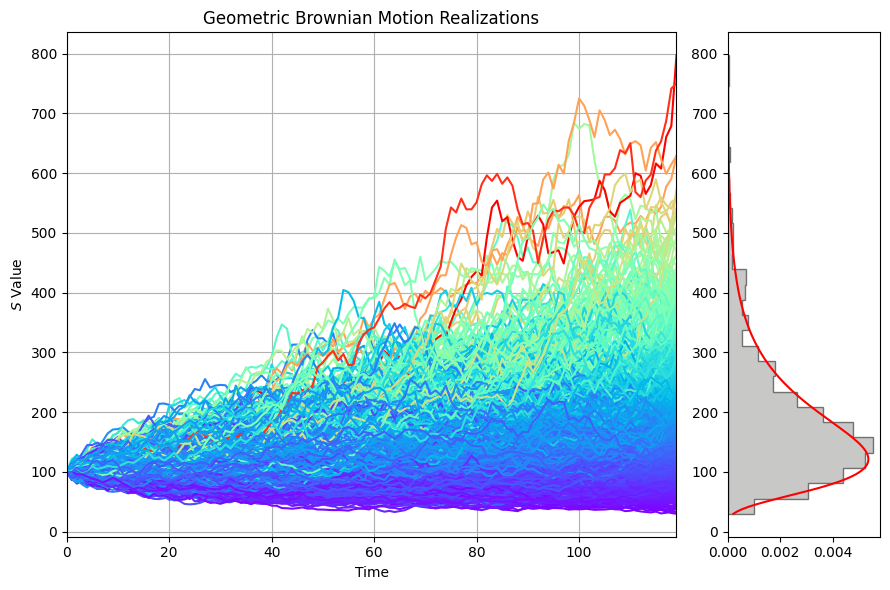
\includegraphics[width=\textwidth]{my_plot}
		\end{columns}
	\end{frame}
\end{document}